\chapter{Patientforløb}

\begin{figure}[H]
\centering
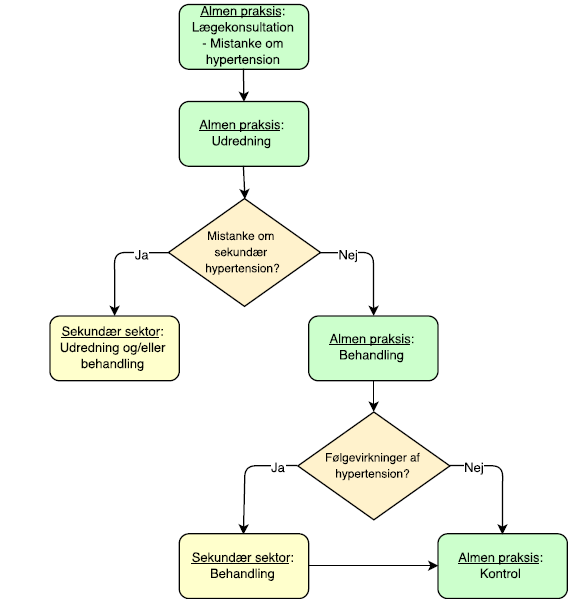
\includegraphics[width=0.9\textwidth]{figures/patientforloeb3}
\caption{Flowchart af patientforløbet fra mistanke om hypertension til behandling og efterfølgende hypertensionskontroller. Illustrationen viser den beslutningstagen, der følger med diagnosticeringen af hypertension, samt sammenspillet mellem sundhedssektorens forskellige dele; almen praksis og den sekundære sektor. De grønne bokse angiver behandling i almen praksis, gule bokse angiver behandling i sekundær sektor, og orange diamantformede bokse angiver beslutninger.}
\label{fig:patientforloeb}
\end{figure}